\documentclass[dvipsnames]{beamer}
\usetheme{Berlin}

\usepackage{epigraph}
\usepackage{xcolor}
\usepackage{amsmath}
\usepackage{tikz}
\usepackage{tikzsymbols}


\setlength\epigraphwidth{.8\textwidth}
\setlength\epigraphrule{0pt}

\newcommand{\pub}[1]{\textcolor{blue}{\texttt{#1}}}
\newcommand{\priv}[1]{\textcolor{brown}{\texttt{#1}}}
\newcommand{\enc}[1]{\colorbox{SkyBlue!75}{\textcolor{white}{\texttt{#1}}}}
\newcommand{\encB}[1]{\colorbox{PineGreen}{\textcolor{white}{\texttt{#1}}}}
\newcommand{\pairing}[3]{e(\enc{#1}, \enc{#2}) $\rightarrow$ \encB{#3}}


\newcommand{\code}[1]{\texttt{#1}}
\newcommand{\keyword}[1]{\textcolor{Violet}{\texttt{#1}}}


% Add a title page for each section
\AtBeginSection[]{
\begin{frame}
    \frametitle{Table of Contents}
    \tableofcontents[currentsection]
\end{frame}
}


\begin{document}
    \title{SNARKS}
    \date{}

    \begin{frame}
        \maketitle

        \epigraph{I ask the fundamental question of rationality: Why do you believe what you believe? What do you think you know and how do you think you know it?}{\textit{Harry Potter\\Harry Potter and the methods of rationality}}
    \end{frame}

    \section{Why?}

    \begin{frame}{Uses of SNARKs}
        \begin{itemize}
            \item SNARKs succinctly prove knowledge of arbitrary statements.
            \item zkSNARKs ensure no additional information is revealed.
            \item For example, you can prove the mere fact that:
            \begin{itemize}
                \item you know the input to a hash function
                \item you created a valid transaction
                \item you donated 10\% of your income to charity
                \item you have enough collateral for a loan
            \end{itemize}
        \end{itemize}
        \qedhere
    \end{frame}


    \section{A zkARK}

    \begin{frame}{Setup}
        \begin{itemize}
            \item Choose a generator \pub{g} and prime \pub{p}
            \item Choose a private key \priv{x}
            \item Calculate the public key \pub{g\priv{$^x$} mod p}
            \item From now on the notation \enc{x} denotes this ``encryption'' operation
        \end{itemize}

        \begin{block}{}
            The goal is to \textbf{demonstrate knowledge} of \priv{x} without revealing it.
        \end{block}
    \end{frame}

    \begin{frame}[plain]{Mathematical tools}
        \begin{block}{Perfect hiding}
            If \priv{r} is a secret random value, \pub{\priv{x} + \priv{r} mod n} is perfectly hidden
        \end{block}

        \pause
        \begin{block}{Partially homomorphic ``encryption''}
            \only<-2>{
            \begin{itemize}
                \item \enc{a}$^c$ = \pub{(g\priv{$^a$})$^c$ mod p} = \pub{g\priv{$^{c\cdot a}$} mod p}= \enc{c$\cdot$a}
                \item \enc{a}*\enc{b} = \pub{g\priv{$^a$} mod p} * \pub{g\priv{$^b$} mod p} = \pub{g\priv{$^{a+b}$} mod p}= \enc{a+b}
            \end{itemize}}
            \only<3->{
            \begin{itemize}
                \item \enc{a}$^c$ = \enc{c$\cdot$a}
                \item \enc{a}*\enc{b} = \enc{a+b}
            \end{itemize}
            }
        \end{block}
    \end{frame}

    \begin{frame}{The Protocol}
        \begin{itemize}
            \item[] \enc{x} is common knowledge.
            \item[] Alice claims to know \priv{x}
        \end{itemize}
        \vspace{1cm}

        \begin{columns}
            \begin{column}{0.5\textwidth}
                \textbf{Alice}
                \begin{itemize}
                    \item[1.] Generates \priv{r}. Sends \enc{r}
                    \item[]
                    \item[3.] Sends \pub{\priv{x} + c$\cdot$r}
                    \item[]
                \end{itemize}
            \end{column}
            \begin{column}{0.5\textwidth}
                \textbf{Bob}
                \begin{itemize}
                    \item[]
                    \item[2.]Generates and sends \pub{c}
                    \item[]
                    \item[4.]Calculates \enc{x + c$\cdot$r} ($\times$2)
                \end{itemize}
            \end{column}
        \end{columns}
    \end{frame}

    \begin{frame}{Extensions}
        \begin{itemize}
            \item We can make this non-interactive by using the Fiat-Shamir heuristic
            \item We can make this into a signature if Alice \textbf{knowingly} uses a hash of the message as the challenge.
        \end{itemize}
    \end{frame}

    \section{Polynomial Computation}

    \begin{frame}{Constraints}
        Consider a function that takes a some inputs and performs a computation. We want to write it as a set of constraints of the form:\\

        \begin{center}
            \priv{c$_n$} = ($\sum_{i=1}^{n-1}$ \pub{r$_i$} \priv{c$_i$}) $\cdot$ ($\sum_{j=1}^{n-1}$ \pub{s$_j$} \priv{c$_j$})\\
            \vspace{0.5cm}
            eg. \priv{c$_5$} = (\priv{c$_1$} + \pub{3}\priv{c$_3$}) $\cdot$ (\pub{2}\priv{c$_1$} + \priv{c$_2$} + \priv{c$_4$})
        \end{center}

        If you know any inputs that cause the function to return the expected value (a witness), then you know a satisfying set of constant \priv{c$_i$} values.
    \end{frame}

    \begin{frame}{An example}
        \begin{columns}
            \begin{column}{0.4\textwidth}
                \code{
                \keyword{def} myFunc(x,y):\\
                \hspace{0.5cm}z = x**2 +y\\
                \hspace{0.5cm}\keyword{return} (x+z)(z+3)
                }
            \end{column}
            \begin{column}{0.6\textwidth}
                c$_1$ = 1\\
                c$_2$ = x\\
                c$_3$ = y\\
                \vspace{0.3cm}
                \hrule
                \vspace{0.3cm}
                c$_4$ = c$_2$ $\cdot$ c$_2$\\
                c$_5$ = (c$_2$ + c$_3$ + c$_4$) $\cdot$ (3c$_1$ + c$_3$ + c$_4$)\\
            \end{column}
        \end{columns}

        \vspace{1cm}
        If the expected output (c$_5$) is 90 then \priv{[1, 2, 3, 4, 90]} is a valid witness.
    \end{frame}

    \begin{frame}{Rank 1 Constraint System}
        Another formulation: represent the first constraint with vectors\\
        \vspace{0.3cm}
        \pub{\begin{bmatrix}
                 0 \\ 1 \\ 0 \\ 0 \\ 0
        \end{bmatrix}}
        \priv{\begin{bmatrix}
                  c$_1$\\ c$_2$\\ c$_3$\\ c$_4$\\ c$_5$
        \end{bmatrix}}
        *
        \pub{\begin{bmatrix}
                 0 \\ 1 \\ 0 \\ 0 \\ 0
        \end{bmatrix}}
        \priv{\begin{bmatrix}
                  c$_1$\\ c$_2$\\ c$_3$\\ c$_4$\\ c$_5$
        \end{bmatrix}}
        =
        \pub{\begin{bmatrix}
                 0 \\ 0 \\ 0 \\ 1 \\ 0
        \end{bmatrix}}
        \priv{\begin{bmatrix}
                  c$_1$\\ c$_2$\\ c$_3$\\ c$_4$\\ c$_5$
        \end{bmatrix}}
        \\

        \vspace{0.6cm}
        c$_4$ = c$_2$ $\cdot$ c$_2$
    \end{frame}

    \begin{frame}{Rank 1 Constraint System}
        Another formulation: represent the second constraint with vectors\\
        \vspace{0.3cm}
        \pub{\begin{bmatrix}
                 0 \\ 1 \\ 1 \\ 1 \\ 0
        \end{bmatrix}}
        \priv{\begin{bmatrix}
                  c$_1$\\ c$_2$\\ c$_3$\\ c$_4$\\ c$_5$
        \end{bmatrix}}
        *
        \pub{\begin{bmatrix}
                 3 \\ 0 \\ 1 \\ 1 \\ 0
        \end{bmatrix}}
        \priv{\begin{bmatrix}
                  c$_1$\\ c$_2$\\ c$_3$\\ c$_4$\\ c$_5$
        \end{bmatrix}}
        =
        \pub{\begin{bmatrix}
                 0 \\ 0 \\ 0 \\ 0 \\ 1
        \end{bmatrix}}
        \priv{\begin{bmatrix}
                  c$_1$\\ c$_2$\\ c$_3$\\ c$_4$\\ c$_5$
        \end{bmatrix}}
        \\

        \vspace{0.6cm}
        c$_5$ = (c$_2$ + c$_3$ + c$_4$) $\cdot$ (3c$_1$ + c$_3$ + c$_4$)
    \end{frame}

    \begin{frame}{Polynomials Recap}
        I'm going to use the term ``polynomial" a lot. A quick recap:

        \begin{center}
            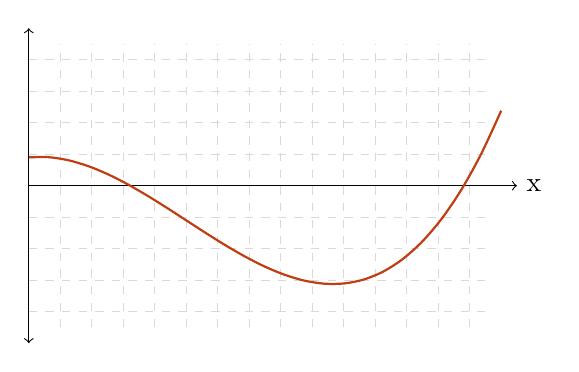
\begin{tikzpicture}[scale=0.4]
                % axis and grid
                \draw[step=1,color=gray!30,dashed] (0,-4.5) grid (14.5,4.5);
                \draw[->] (0,0) -- (15.5,0) node[right] {x};
                \draw[<->] (0,-5) -- (0,5);

                \draw [smooth,domain=0:15,thick,Bittersweet] plot (\x,{0.01 * \x^3 - 0.15 * \x^2 + 0.1 * \x + 0.9});
            \end{tikzpicture}\\
            P(x) = a$_0$ + a$_1$x + a$_2$x$^2$ + a$_3$x$^3$
        \end{center}
    \end{frame}

    \begin{frame}{Quadratic Arithmetic Program}
        Another formulation: represent all constraints with polynomials\\
        Start by representing each constraint as a value on the x-axis and then create some basis polynomials to isolate each constraint\\

        \begin{center}
            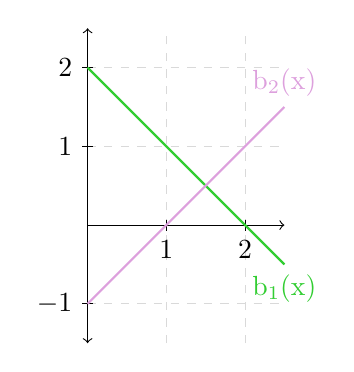
\begin{tikzpicture}
                % axis and grid
                \draw[step=1,color=gray!30,dashed] (0,-1.5) grid (2.5,2.5);
                \draw[->] (0,0) -- (2.5,0);
                \draw[<->] (0,-1.5) -- (0,2.5);

                \foreach \x/\xtext in {1/1, 2/2}
                \draw[shift={(\x,0)}] (0pt,2pt) -- (0pt,-2pt) node[below] {$\xtext$};
                \foreach \y/\ytext in {-1/-1, 1/1, 2/2}
                \draw[shift={(0,\y)}] (2pt,0pt) -- (-2pt,0pt) node[left] {$\ytext$};

                \draw [smooth,domain=0:2.5,thick,LimeGreen] plot (\x,{2 - \x}) node[below] {b$_1$(x)};
                \draw [smooth,domain=0:2.5,thick,Plum] plot (\x,{\x - 1}) node[above] {b$_2$(x)};
            \end{tikzpicture}
        \end{center}

    \end{frame}

    \begin{frame}{Quadratic Arithmetic Program}
        Encode the constraints as a polynomial equation\\

        \begin{align*}
            c_4 &= c_2 \cdot c_2\\
            c_5 &= (c_2 + c_3 + c_4) \cdot (3c_1 + c_3 + c_4)\\
            \\
            \textcolor{LimeGreen}{b_1(x)} &= R_2 = O_4\\
            \textcolor{Plum}{b_2(x)} &= L_3 = L_4 = R_1 = R_3 = R_4 = O_5\\
            \textcolor{LimeGreen}{b_1(x)} + \textcolor{Plum}{b_2(x)} &= L_2\\
            0 &= L_1 = L_5 = R_5 = O_1 = O_2 = O_3\\
        \end{align*}\\

        \begin{center}
            \priv{L} = $\sum_{i=1}^{5}$ \priv{c$_i$}\pub{r$_i$L$_i$} \hspace{0.3cm}
            \priv{R} = $\sum_{i=1}^{5}$ \priv{c$_i$}\pub{s$_i$R$_i$} \hspace{0.3cm}
            \priv{O} = $\sum_{i=1}^{5}$ \priv{c$_i$}\pub{O$_i$}
        \end{center}
    \end{frame}

    \begin{frame}{Completed QAP}
        \textcolor{LimeGreen}{b$_1$(x)} = 2 - x \\
        \textcolor{Plum}{b$_2$(x)} = x - 1\\
        \priv{L} = \priv{c$_2$}\textcolor{LimeGreen}{b$_1$(x)} + (\priv{c$_2$} + \priv{c$_3$} + \priv{c$_4$})\textcolor{Plum}{b$_2$(x)} \\
        \priv{R} = \priv{c$_2$}\textcolor{LimeGreen}{b$_1$(x)} + (3\priv{c$_1$} + \priv{c$_3$} + \priv{c$_4$})\textcolor{Plum}{b$_2$(x)} \\
        \priv{O} = \priv{c$_4$}\textcolor{LimeGreen}{b$_1$(x)} + \priv{c$_5$}\textcolor{Plum}{b$_2$(x)}\\
        \vspace{0.5cm}

        \begin{block}{}
            \priv{P}(x) = \priv{L}(x) * \priv{R}(x) - \priv{O}(x)\\
            In the satisfying case \priv{P}(1) = \priv{P}(2) = 0
        \end{block}
    \end{frame}

    \section{SARKs}

    \begin{frame}{Building blocks}
        We can recast our partially homomorphic ``encryption'' procedure to use an Elliptic curve group
        \begin{itemize}
            \item c$\cdot$\enc{a} = \enc{c$\cdot$a}
            \item \enc{a} + \enc{b} = \enc{a + b}
        \end{itemize}


        Note that it lets anyone produce linear combinations of encrypted values.

        We will also make use of a closely related elliptic curve group
    \end{frame}

    \begin{frame}{Building blocks}
        The knowledge of coefficient test
        \vspace{0.5cm}

        \begin{columns}
            \begin{column}{0.4\textwidth}
                \textbf{Alice}
                \begin{itemize}
                    \item[]
                    \item[]
                    \item Generates \enc{X} != \enc{a}
                    \item Returns (\enc{X}, \enc{$\alpha \cdot$X})
                    \item[]
                \end{itemize}
            \end{column}
            \begin{column}{0.6\textwidth}
                \textbf{Bob}
                \begin{itemize}
                    \item Generates \priv{$\alpha$} and \priv{a}
                    \item Sends (\enc{a}, \enc{$\alpha \cdot$a})
                    \item[]
                    \item[]
                    \item Confirms returned pair is valid
                \end{itemize}
            \end{column}
        \end{columns}
        \begin{center}
            How can she do this?\\
            \pause
            Alice returned a transformation \enc{X} = \enc{d$\cdot$a}
        \end{center}
    \end{frame}

    \begin{frame}{Building blocks}
        The extended knowledge of coefficient test
        \vspace{0.5cm}

        \begin{columns}
            \begin{column}{0.4\textwidth}
                \textbf{Alice}
                \begin{itemize}
                    \item[]
                    \item[]
                    \item Generates new \enc{X}
                    \item Returns (\enc{X}, \enc{$\alpha \cdot$X})
                    \item[]
                \end{itemize}
            \end{column}
            \begin{column}{0.6\textwidth}
                \textbf{Bob}
                \begin{itemize}
                    \item Generates \priv{$\alpha$}, \priv{a}, \priv{b}, \priv{c}, ...
                    \item Sends (\enc{a}, \enc{$\alpha \cdot$a}, \enc{b}, \enc{$\alpha \cdot$b}, ...)
                    \item[]
                    \item[]
                    \item[] \item Confirms returned pair is valid
                \end{itemize}
            \end{column}
        \end{columns}
        \begin{center}
            How can she do this?\\
            \pause
            Alice returned a linear combination of \enc{a}, \enc{b}, \enc{c}, ...
        \end{center}
    \end{frame}

    \begin{frame}{Building blocks}
        Blind verification of a polynomial
        \vspace{0.5cm}

        \begin{columns}
            \begin{column}{0.4\textwidth}
                \textbf{Alice}
                \begin{itemize}
                    \item[]
                    \item[]
                    \item Generates new \enc{X}
                    \item Returns (\enc{X}, \enc{$\alpha \cdot$X})
                    \item[]
                \end{itemize}
            \end{column}
            \begin{column}{0.6\textwidth}
                \textbf{Bob}
                \begin{itemize}
                    \item Generates \priv{$\alpha$}, \priv{s}
                    \item Sends (\enc{1}, \enc{$\alpha$}, \enc{s}, \enc{$\alpha \cdot$s}, \enc{s$^2$}, ...)
                    \item[]
                    \item[]
                    \item[] \item Confirms returned pair is valid
                \end{itemize}
            \end{column}
        \end{columns}
        \begin{center}
            Alice returned an encrypted polynomial in x, evaluated at \priv{s}\\
            \enc{X} = \enc{a$_0$ + a$_1$s + a$_2$s$^2$ + a$_3$s$^3$}
        \end{center}
    \end{frame}

    \begin{frame}{Simplifying the problem}
        Recall the QAP:
        \begin{itemize}
            \item We have constructed a polynomial equation\\\priv{P}(x) = \priv{L}(x)\priv{R}(x) - \priv{O}(x)
            \item Someone who knows a satisfying assignment can choose \priv{L}, \priv{R} and \priv{O} such that \priv{P}(1) = 0 and \priv{P}(2) = 0
        \end{itemize}
        Re-framing the condition:
        \begin{itemize}
            \item \priv{P}(x) = \priv{H}(x)\pub{Z}(x) where \pub{Z}(x) = (x-1)(x-2). \\Note that this is equation holds for all x
            \item In practice, we only need to demonstrate knowledge of a solution at a \textbf{secret} point \priv{s}.
            Without knowing \priv{P} or \priv{s}, it is difficult to produce P' and H' such that P'(s) = H'(s)\pub{Z}(s)
        \end{itemize}
    \end{frame}

    \begin{frame}{Verifying satisfying polynomials}
        \begin{itemize}
            \item The goal is for Alice to demonstrate she knows \priv{L}, \priv{R}, \priv{O} and \priv{H}.
            \item We already have a way to verify polynomial \priv{H}. For the others, we want to ensure it is a \textit{satisfying} polynomial
            \item Recall \priv{L} = \priv{c$_1$}\pub{L$_1$} + \priv{c$_2$}\pub{L$_2$} + \priv{c$_3$}\pub{L$_3$} + \priv{c$_4$}\pub{L$_4$} +\priv{c$_5$}\pub{L$_5$}
            \item So Bob should send \enc{L$_1$(s)}, \enc{$\beta\cdot$L$_1$(s)}, \enc{L$_2$(s)}, \enc{$\beta\cdot$L$_2$(s)}, ...
            \item Then Alice can return a putative \enc{L(s)} (and \enc{$\beta\cdot$L(s)})
            \item Similarly, if Bob sends \enc{R$_1$(s)}, \enc{$\gamma\cdot$3R$_1$(s)}, ..., \enc{O$_1$(s)}, \enc{$\delta\cdot$O$_1$(s)}, ..., Alice can return a putative \enc{R(s)} and \enc{O(s)}
        \end{itemize}
    \end{frame}

    \begin{frame}{Verifying simultaneous satisfying polynomials}
        The described solution does not actually verify that the returned \enc{L(s)}, \enc{R(s)} and \enc{O(s)} values use the same coefficients. To achieve this, we can add another step to the protocol:
        \begin{itemize}
            \item Bob sends \enc{(L$_1$+R$_1$+O$_1$)(s)}, \enc{$\epsilon$\cdot(L$_1$+R$_1$+O$_1$)(s)}, ...
            \item Alice returns \enc{L(s)+R(s)+O(s)}
            \item Bob checks that this value matches \enc{L(s)}+\enc{R(s)}+\enc{O(s)}
            \item The logic here is that if the individual polynomials were constructed using different coefficients, Alice could not recreate their sum as a linear combination of the (\pub{L$_i$}+\pub{R$_i$}+\pub{O$_i$})(\priv{s}) values
        \end{itemize}
    \end{frame}

    \begin{frame}{Pinocchio Protocol}
        So now we can (almost) construct a SARK:
        \begin{itemize}
            \item Alice claims to know satisfying polynomials \priv{L}, \priv{R}, \priv{O} and \priv{H} such that \priv{LR} - \priv{O} = \priv{H}\pub{Z}
            \item Bob chooses a private point \priv{s}
            \item Alice sends \enc{L(s)}, \enc{R(s)}, \enc{O(s)} and \enc{H(s)} using the known procedure, which convinces Bob that all polynomials are legitimately constructed.
            \item  Lastly, Bob should confirm that\\
            \enc{L(s)} * \enc{R(s)} - \enc{O(s)} = \enc{Z(s)} * \enc{H(s)}
            \\He can't check this directly because our ``encryption" scheme does not support multiplication.
        \end{itemize}
    \end{frame}

    \begin{frame}{Elliptic Curve Pairing}
        \begin{block}{}
            Define a pairing from the elliptic curve group to a related group
            \begin{center}
                \pairing{a}{b}{ab}
            \end{center}
        \end{block}

        \begin{itemize}
            \item Note that we're multiplying \textbf{coefficients} (not group elements)
            \item The result is in a new group so we can't apply it recursively
        \end{itemize}
    \end{frame}

    \begin{frame}{Checking the polynomial equation}
        Bob has putative values for each term and he wants to confirm:\\
        \begin{center}
            \enc{L(s)} * \enc{R(s)} = \enc{Z(s)} * \enc{H(s)} + \enc{O(s)}
        \end{center}

        \begin{itemize}
            \item \pairing{L(s)}{R(s)}{L(s)R(s)}
            \item \pairing{Z(s)}{H(s)}{Z(s)H(s)}
            \item \pairing{1}{O(s)}{O(s)}
            \item \encB{Z(s)H(s)} * \encB{O(s)} =  \encB{Z(s)H(s) + O(s)}
        \end{itemize}
    \end{frame}

    \begin{frame}{CELEBRATE}
        \vspace{2.5cm}
        \begin{center}
        {\Huge You can create a SARK$^*$}
            \\
        \end{center}

        \vspace{2.5cm}
        {\tiny $^*$Succinct for the prover}
    \end{frame}

    \section{SNARKs}

    \begin{frame}{Non-interactive proofs}
        Recall that in the interactive protocol, Bob needs to:
        \begin{itemize}
            \item Generate \priv{s} and publish encrypted powers: \enc{1}, \enc{s}, \enc{s$^2$}, ...
            \item Publish lots of polynomials evaluated at \priv{s}:\\
            \enc{L$_i$(s)}, \enc{R$_i$(s)}, \enc{O$_i$(s)}, \enc{(L$_i$+R$_i$+O$_i$)(s)}, \enc{Z(s)}
            \item Generate \priv{$\alpha$}, \priv{$\beta$}, \priv{$\gamma$} and publish encrypted shifts:\\
            \enc{$\alpha \cdot$s$^i$}, \enc{$\beta \cdot$L$_i$(s)}, \enc{$\gamma \cdot$R$_i$(s)}, \enc{$\delta \cdot$O$_i$(s)}, \enc{$\epsilon \cdot$(L$_i$+R$_i$+O$_i$)(s)}
            \item Everyone else is in the same position as Alice - they could use the same values for their proof.
            \item If Bob deletes the private values, all proofs are non-interactive
            \item As a security measure, we generate them collaboratively
        \end{itemize}
    \end{frame}

    \begin{frame}{Non-interactive verification}
        \begin{itemize}
            \item[] In the interactive protocol, Bob verifies shifts directly: given putative \enc{H(x)} and \enc{$\alpha \cdot$H(x)} values, he calculates \priv{$\alpha$}\enc{H(x)} to see if it matches \enc{$\alpha \cdot$H(x)}
            \item[] However, a generic verifier can compare the elliptic curve pairings:
            \begin{itemize}
                \item \pairing{$\alpha$}{H(x)}{$\alpha \cdot$H(x)}
                \item \pairing{1}{$\alpha \cdot$H(x)}{$\alpha \cdot$H(x)}
            \end{itemize}
        \end{itemize}
    \end{frame}


    \section{zkSNARKs}

    \begin{frame}
        Alice's encrypted polynomials may leak part of her assignment\\
        \vspace{0.6cm}

        Instead, she can use perfect hiding with random offsets:
        \begin{itemize}
            \item L$_z$ = L + $\Delta_L \cdot$Z
            \item R$_z$ = R + $\Delta_R \cdot$Z
            \item O$_z$ = O + $\Delta_O \cdot$Z
        \end{itemize}
        \vspace{0.6cm}

        Since these modifications are multiples of Z\\
        L$_z$ * R$_z$ - O$_z$ is still a multiple of Z
    \end{frame}

    \section{External constraints}

    \begin{frame}{External constraints}
        How can we enforce constraints like c$_1$=1 or c$_5$=90?
        Make the verifier choose the values.

        \begin{itemize}
            \item Consider Alice's encrypted polynomial\\
            \enc{L(s)} = \enc{(c$_1$L$_1$ + c$_2$L$_2$ + c$_3$L$_3$ + c$_4$L$_4$ + c$_5$L$_5$)(s)}
            \item If \enc{$\beta\cdot$L$_5$} is not published then the \enc{c$_5$L$_5$} term cannot exist
            \item The verifier can just add \enc{90L$_5$} to complete the polynomial
            \item This effectively forces the constraint \pub{c$_5$} = 90
        \end{itemize}
    \end{frame}

    \begin{frame}{fin}

    {\huge Questions / Comments / Criticisms?}
    \end{frame}

\end{document}

